\documentclass{zkdl-presentation-template}

% Bibliography
\usepackage[backend=biber]{biblatex}
\bibliography{bibliography.bib}

\usepackage{tabularx}

% Include subfigure package
\usepackage{subfigure}
\usepackage{subcaption}

% Numeration
\addtobeamertemplate{navigation symbols}{}{%
    \usebeamerfont{footline}%
    \usebeamercolor[fg]{footline}%
    \hspace{1em}%
    \textbf{\insertframenumber/\inserttotalframenumber}
    \vspace{3.5px}
}

\title[Математичні основи нейронних мереж]{\textbf{Математичні Основи Штучних
Нейронних Мереж}} 

\author{Виконав: Захаров Дмитро Олегович\inst{1} \\ Науковий керівник: Ігнатович Світлана Юріївна\inst{2}} 

\institute[shortinst]{
    \inst{1} Студент групи МП41 IV курсу (перший бакалаврський рiвень), спецiальностi 113
``Прикладна математика'' освiтньої програми ``Прикладна математика''.\\
    \inst{2} Доктор фiз.-мат. наук, професор кафедри прикладної математики.
}

\date{25 листопада 2024}

\begin{document}
    \frame {
      \titlepage 
      %\hfill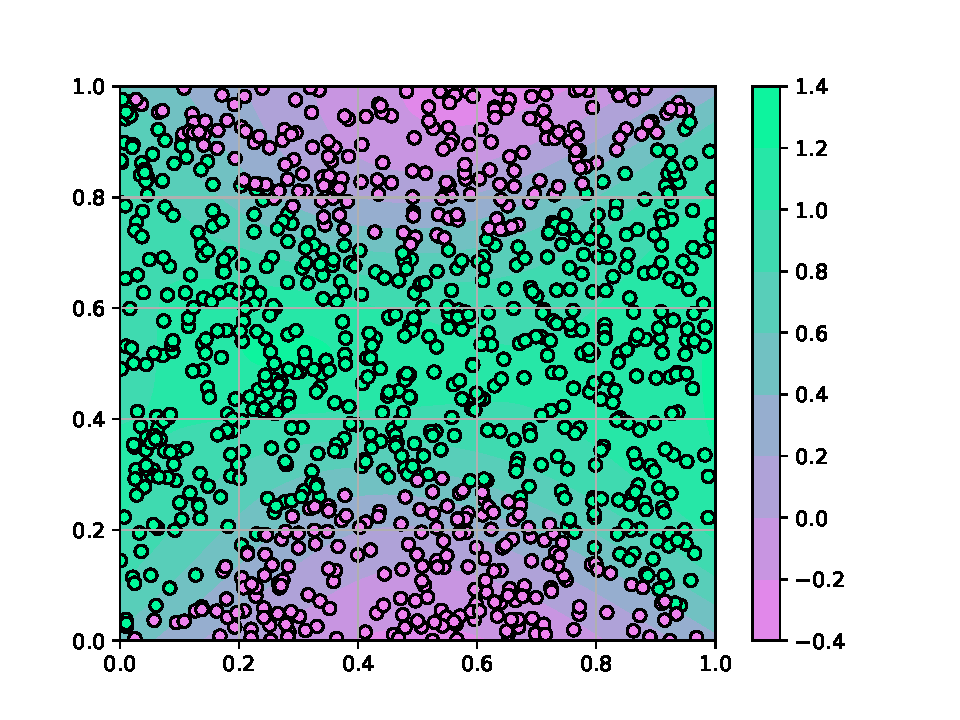
\includegraphics[trim={1.75cm 2.0cm 3.75cm 1cm},clip,width=0.4\textwidth]{../code/classification-cont-prediction.pdf}
    }
  
    \begin{frame}{План}
      \tableofcontents
    \end{frame}

    \section[Вступ]{Вступ: Задачі Глибокого Навчання}
    % \begin{frame}{Навіщо машинне навчання?}		
	% 	\begin{columns}
    %     % Description
    %     \begin{column}{0.5\textwidth}
    %         \begin{itemize}
    %             \item До якогось моменту, нам вистачало класичних методів: ми легко аналізуємо будь-які лінійні, поліноміальні залежності, апроксимуємо одновимірні функції...
    %             \item Проте, з якогось моменту, задачі стали складніші: обробка зображень, текстів, голосу, генерація музики, текстів, зображень... 
    %             \item Це вимагає функцій з дуже багатьма вимірами і величезною складністю залежностей. 
    %         \end{itemize}
    %     \end{column}
    %     % Column 2    
    %     \begin{column}{0.5\textwidth}
    %         \begin{figure}
    %         \centering
    %             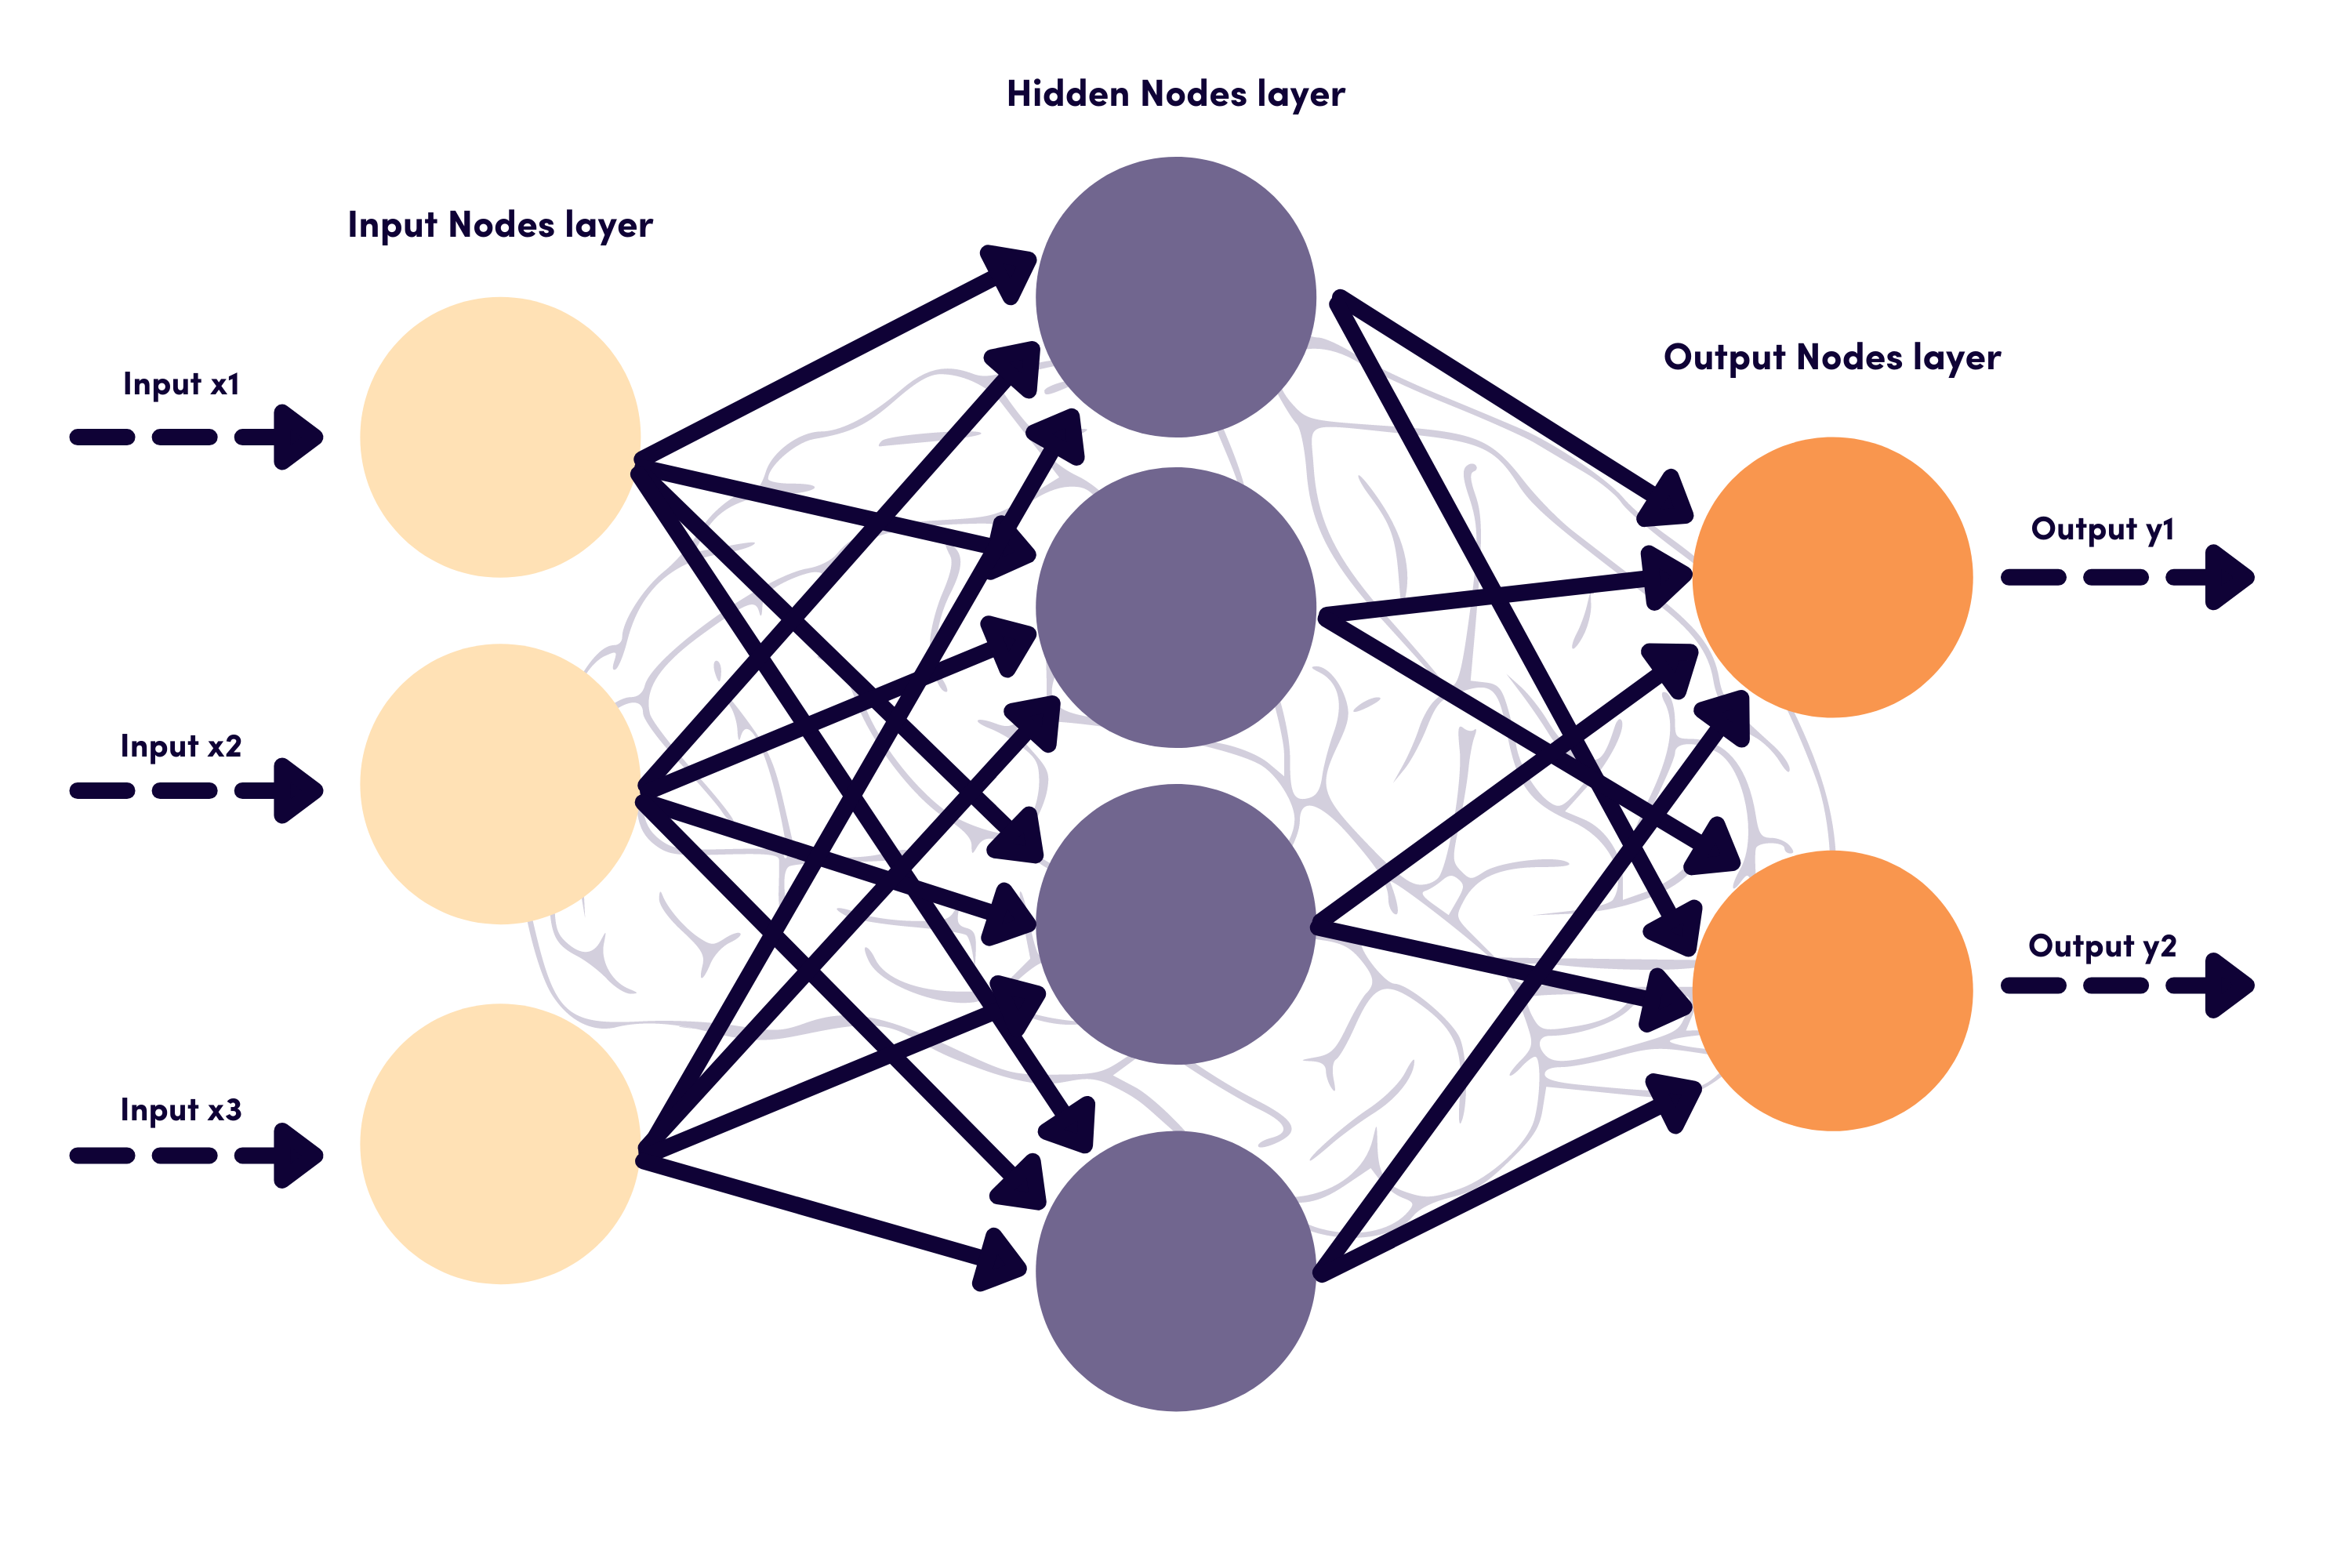
\includegraphics[width=1\textwidth]{images/web.png}
    %         \end{figure}
    %     \end{column}
    %     \end{columns}
	% \end{frame}

    % \begin{frame}{Застосування}
    %     \begin{enumerate}
    %         \item Рекомендаційні системи.
    %         \item Обробка природних мов.
    %         \item Аналіз біометрії.
    %         \item Генерація зображень.
    %         \item Детекція об'єктів.
    %         \item ...
    %     \end{enumerate}
    % \end{frame}

    % \begin{frame}{Глибоке навчання це весело: Pix2Pix}
	%     \begin{figure}
    %     \centering
    %         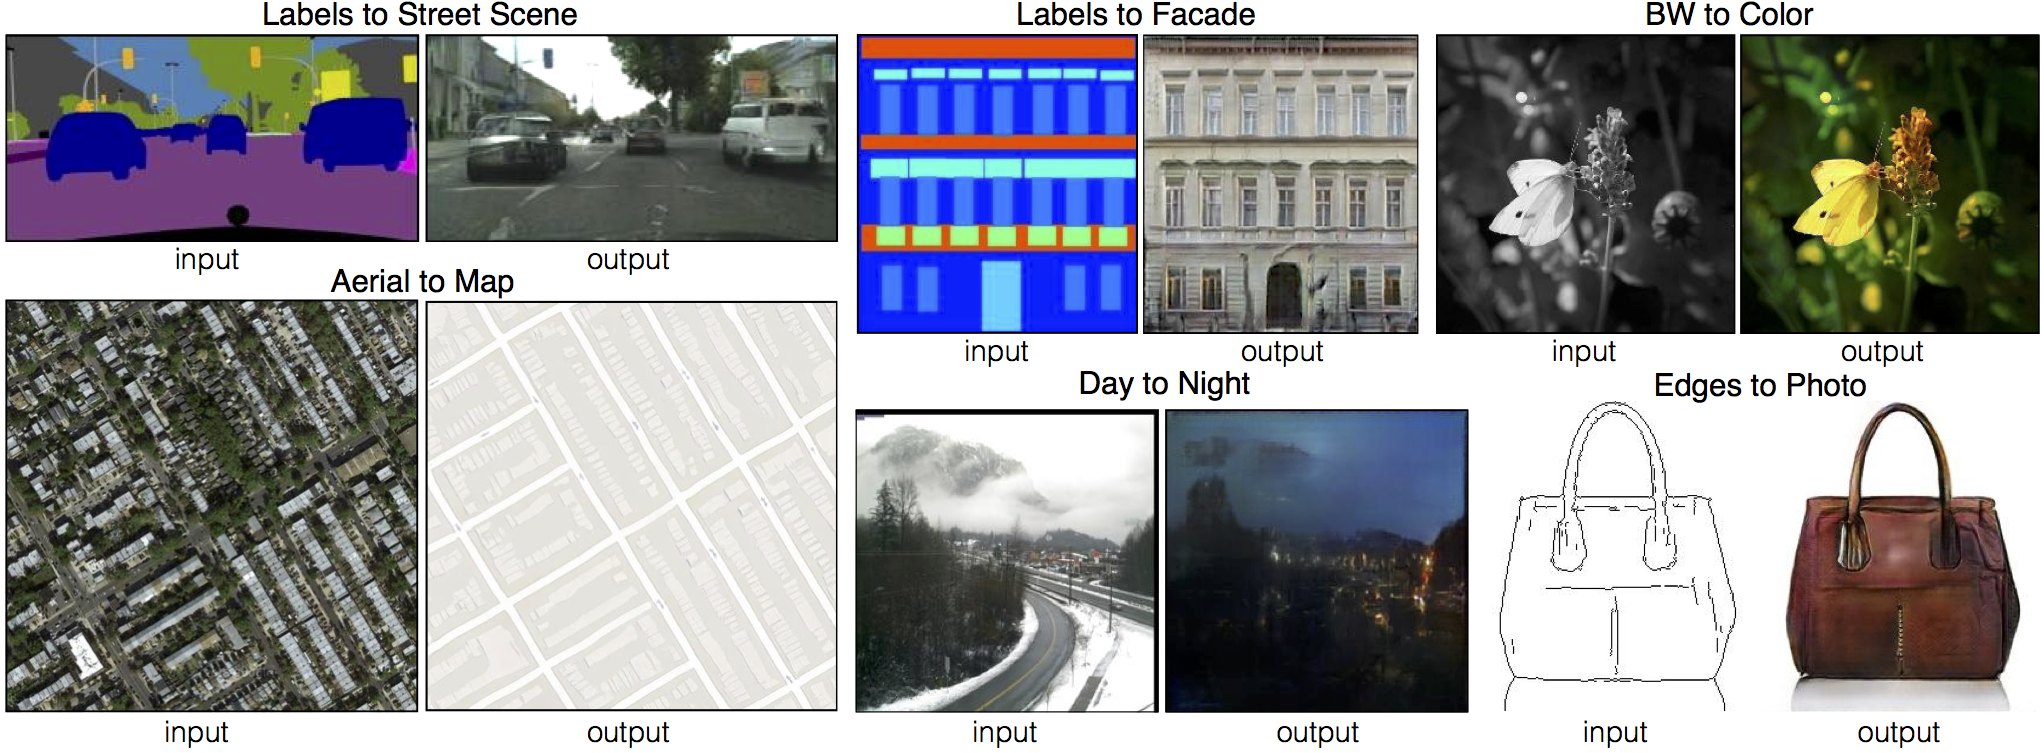
\includegraphics[width=\textwidth]{images/pix2pix.png}
    %         \caption{Трансформація зображення у зображення. \textit{Pix2Pix}.
    %         Більше інформації можна знайти за посиланням:
    %         \href{https://phillipi.github.io/pix2pix/}{phillipi.github.io/pix2pix/}}
    %     \end{figure}
	% \end{frame}

    %  \begin{frame}{Глибоке навчання це весело: Neural Transfer}
	%     \begin{figure}
    %     \centering
    %         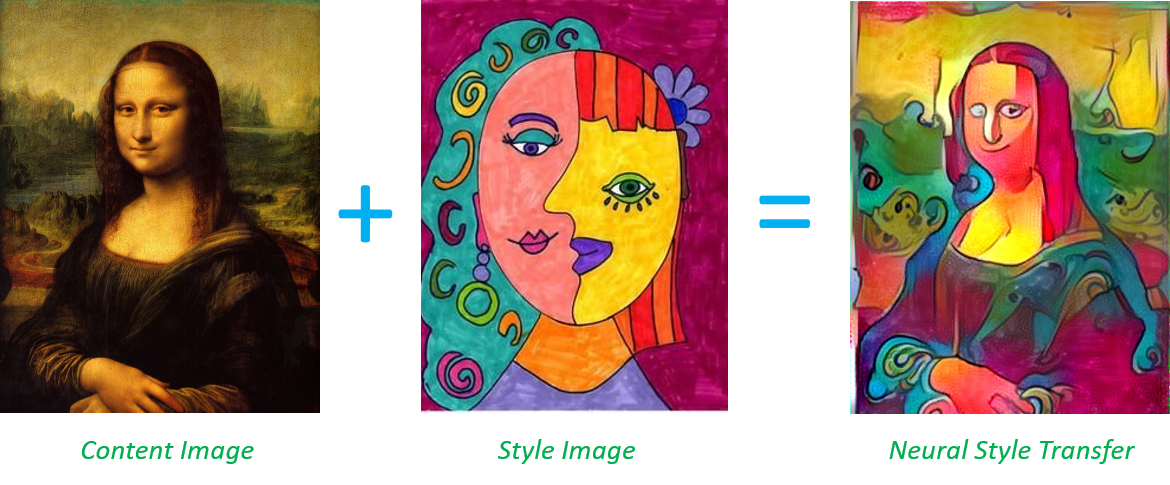
\includegraphics[width=\textwidth]{images/neural-transfer.png}
    %         \caption{Нейронний Перенос. Більше інформації можна знайти за
    %         посиланням
    %         \href{https://www.v7labs.com/blog/neural-style-transfer}{https://www.v7labs.com/blog/neural-style-transfer}.}
    %     \end{figure}
	% \end{frame}

    %  \begin{frame}{Глибоке навчання це весело: ChatGPT}
	%     \begin{figure}
    %     \centering
    %         
\includegraphics[width=\textwidth]{images/chatgpt.jpg}
    %         \caption{Думаю, в представлені не потребується.}
    %     \end{figure}
	% \end{frame}

    \subsection{Приклади}
    \begin{frame}{Опис типової задачі}
        \begin{alertblock}{Проблема}
            Сучасний розвиток інструментів зводить розв'язок задач машинного
            навчання до вибору архітектури моделі, функції втрати та метрик
            якості. Часто, опускається фундаментальне питання: чому ці
            архітектури взагалі працюють?\pause
        \end{alertblock}

        \begin{itemize}
            \item На вхід подається певний набір даних $\mathcal{D}$.
            Найчастіше, це набір пар $\{(\boldsymbol{x}_n,\boldsymbol{y}_n)\}_{1
            \leq n \leq N}$ (\textit{supervised learning}).\pause
            \item Ми віримо, що є певна інформація, яку ми хочемо здобути з цього набору. Ми інкапсулюємо цю інформацію у вигляді функції $f(\boldsymbol{x})$. Це і є \textbf{модель}.\pause
            \item Функцію $f$ ми маємо підібрати з певного класу $\mathcal{F}$ так, щоб за неї досягався певний мінімум ($\hat{f} := \argmin_{f \in \mathcal{F}}\mathcal{L}(\mathcal{D}|f)$).
        \end{itemize}
    \end{frame}

    \begin{frame}{Приклади}
        У попередніх наших роботах
        \cite{our-biometrics-1,our-biometrics-2,our-biometrics-3} ми, зокрема,
        досліджували задачу кібербезпеки біометричних даних:

        \begin{table}
            \scriptsize
            \centering
            \begin{tabularx}{\textwidth}{|c|X|X|X|}
                \hline
                \cellcolor{gray!20}\textbf{Робота} & \cellcolor{gray!20}\textbf{Рік, Журнал} & \cellcolor{gray!20}\textbf{Модель} & \cellcolor{gray!20}\textbf{Набір даних} \\
                \cite{our-biometrics-1} & 2023, Multimedia Tools and Applications (Springer) & $f: \mathcal{I} \to \{0,1\}^{128}$: Бінарний вектор характеристик & Набір зображень і ідентифікатор людей \\
                \cite{our-biometrics-2} & 2024, Computers \& Security (Elsevier) & $f: \mathcal{I} \to \{0,1\}$: Класифікатор живності & Набір зображень і біт, чи фейкова людина \\
                \cite{our-biometrics-3} & 2024, Engineering Applications of AI (Elsevier) & $f: \mathcal{I} \to \mathcal{I}$: ``Геш'' значення фотографії людини & Набір зображень і ідентифікатор людей \\
                \hline
            \end{tabularx}
            \caption{Приклади наших робіт з біометрії. $\mathcal{I}$ --- множина зображень.}
        \end{table}

        \pause\begin{alertblock}{Проте...}
            Усі ці задачі містять багатовимірні дані (вимірність $\geq 100000$), які важко апроксимувати
            класичними методами. Отже, ми використовуємо \textbf{глибоке навчання}.
        \end{alertblock}
    \end{frame}

    \subsection{Проблема параметризації}
    \begin{frame}{Параметризація моделі}
        \begin{block}{Зауваження}
            Як на практиці має виглядати $\mathcal{F}$? Зауважимо --- це не може
            бути щось на кшталт $L^2(\mathbb{R})$. Тому, ми
            \textbf{параметризуємо} модель параметрами $\boldsymbol{\theta} \in
            \Theta \subset \mathbb{R}^n$. Записуємо це як
            $f(\boldsymbol{x}|\boldsymbol{\theta})$.\pause
        \end{block}

        \begin{example}
            Якщо ми віримо, що $f: \mathbb{R} \to \mathbb{R}$ --- квадратична, то
            шукаємо $f$ як:
            \begin{equation*}
                f(x|\boldsymbol{\theta}) = \theta_2 x^2 + \theta_1 x + \theta_0, \quad \boldsymbol{\theta} = (\theta_0, \theta_1, \theta_2) \in \mathbb{R}^3.
            \end{equation*}
        \end{example}

        \pause\begin{example}[Багатовимірна лінійна регресія]
            Нехай $\mathcal{D} = \{(\boldsymbol{x}_n,y_n)\}_{1 \leq n \leq N}
            \subset \mathbb{R}^d \times \mathbb{R}$. Моделлю може бути наступна
            лінійна функція
            \begin{equation*}
                f(\boldsymbol{x}|\boldsymbol{\theta}) = \boldsymbol{w}^{\top} \boldsymbol{x} + \beta, \quad \boldsymbol{\theta} = (\boldsymbol{w}, \beta) \in \mathbb{R}^{d+1}.
            \end{equation*}
        \end{example}
    \end{frame}

    \begin{frame}
        \begin{block}{Зауваження}
            Модель --- це не завжди функція, що повертає скаляр/вектор. Модель
            може повертати і зображення/аудіо/репрезентацію тексту/ймовірністний
            розподіл.\pause
        \end{block}

        Так чи інакше, ми маємо функцію втрати $\mathcal{L}(\mathcal{D}|\boldsymbol{\theta})$, що вимірює, наскільки добре модель описує дані. Правило вибору параметрів:
        \begin{equation*}
            \hat{\boldsymbol{\theta}} := \argmin_{\boldsymbol{\theta} \in \Theta} \mathcal{L}(\mathcal{D}|\boldsymbol{\theta}).
        \end{equation*}
        \vspace{-15px}
        \pause\begin{example}[Багатовимірна лінійна регресія]
            Нехай $\mathcal{D} = \{(\boldsymbol{x}_n,\boldsymbol{y}_n)\}_{1 \leq
            n \leq N} \subset \mathbb{R}^d \times \mathbb{R}^r$. Тоді, ми можемо
            обирати
            $f(\boldsymbol{x}|\boldsymbol{W},\boldsymbol{\theta})=\boldsymbol{W}\boldsymbol{x}+\boldsymbol{\beta}$ таким чином,
            щоб $f(\boldsymbol{x}_n) \approx \boldsymbol{y}_n$ для всіх $n$. Тому, в якості функції втрати можна взяти:\pause
            
            \vspace{-20px}
            \begin{align*}
                \mathcal{L}(\mathcal{D}|\boldsymbol{W},\boldsymbol{\theta}) &= \frac{1}{N}\sum_{n=1}^N\left\|f(\boldsymbol{x}_n|\boldsymbol{W},\boldsymbol{\theta}) - \boldsymbol{y}_n \right\|^2.
            \end{align*}
        \end{example}
    \end{frame}

    \begin{frame}{Візуалізація}
    \begin{figure}
        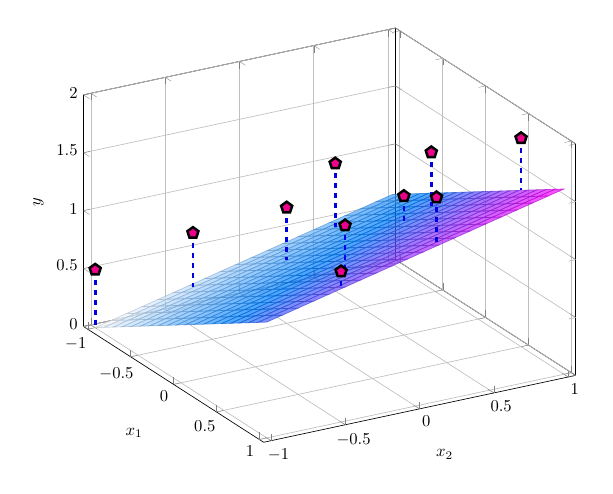
\begin{tikzpicture}[scale=0.6]
            % Define the 3D plot
            \begin{axis}[
                view={60}{30}, % Angle for 3D view
                xlabel={$x_1$},
                ylabel={$x_2$},
                zlabel={$y$},
                domain=-1:1,
                samples=20,
                width=12cm,
                grid=both,
                zmin=0, zmax=2,
                xmin=-1.05, xmax=1.05,
                ymin=-1.05, ymax=1.05,
                colormap/cool
            ]
        
            % Plot the regression plane
            \addplot3[surf, opacity=0.7] {0.5*x + 0.3*y + 0.8};
        
            % Add sample data points
            \addplot3[only marks, mark=pentagon*, fill=magenta, mark size=3.5pt, line width=1.5pt] coordinates {
                (-1, -1, 0.5)
                (-0.8, 0.5, 1.1)
                (-0.5, 0, 1)
                (-0.2, 0.8, 1.4)
                (0, 0.5, 1.2)
                (0.5, 1, 1.8)
                (0.7, -0.3, 1.5)
                (0.9, 0.2, 1.7)
                (1, -0.5, 1.3)
                (-0.9, -0.4, 0.7)
            };
        
            % Add red dashed projection lines without labels
            \addplot3[blue!90!black, ultra thick, dashed] coordinates {(-1, -1, 0.5) (-1, -1, {0.5*-1 + 0.3*-1 + 0.8})};
            \addplot3[blue!90!black, ultra thick, dashed] coordinates {(-0.8, 0.5, 1.1) (-0.8, 0.5, {0.5*-0.8 + 0.3*0.5 + 0.8})};
            \addplot3[blue!90!black, ultra thick, dashed] coordinates {(-0.5, 0, 1) (-0.5, 0, {0.5*-0.5 + 0.3*0 + 0.8})};
            \addplot3[blue!90!black, ultra thick, dashed] coordinates {(-0.2, 0.8, 1.4) (-0.2, 0.8, {0.5*-0.2 + 0.3*0.8 + 0.8})};
            \addplot3[blue!90!black, ultra thick, dashed] coordinates {(0, 0.5, 1.2) (0, 0.5, {0.5*0 + 0.3*0.5 + 0.8})};
            \addplot3[blue!90!black, ultra thick, dashed] coordinates {(0.5, 1, 1.8) (0.5, 1, {0.5*0.5 + 0.3*1 + 0.8})};
            \addplot3[blue!90!black, ultra thick, dashed] coordinates {(0.7, -0.3, 1.5) (0.7, -0.3, {0.5*0.7 + 0.3*-0.3 + 0.8})};
            \addplot3[blue!90!black, ultra thick, dashed] coordinates {(0.9, 0.2, 1.7) (0.9, 0.2, {0.5*0.9 + 0.3*0.2 + 0.8})};
            \addplot3[blue!90!black, ultra thick, dashed] coordinates {(1, -0.5, 1.3) (1, -0.5, {0.5*1 + 0.3*-0.5 + 0.8})};
            \addplot3[blue!90!black, ultra thick, dashed] coordinates {(-0.9, -0.4, 0.7) (-0.9, -0.4, {0.5*-0.9 + 0.3*-0.4 + 0.8})};

            % Label axes
            %\node at (axis cs: 1, 0, 2) [anchor=north west] {Regression Plane};
            %\node at (axis cs: -1, -1, 0) [anchor=north] {Data Points};
            %\node at (axis cs: -1, 1, 1.5) [anchor=west, rotate=15] {Error Lines (Loss)};
            
            \end{axis}
        \end{tikzpicture}
        \caption{Приклад багатовимірної лінійної регресії для $\boldsymbol{x}_n
        \in \mathbb{R}^2$, $y_n \in \mathbb{R}$. Ціль підібрати площину
        $f(\boldsymbol{x}|\beta,w_1,w_2) := \beta+w_1x_1+w_2x_2$ так, щоб
        втрата $\mathcal{L}(\mathcal{D}|\beta,w_1,w_2)=\frac{1}{N}\sum_{n=1}^N\textcolor{blue!90!black}{\|f(\boldsymbol{x}_n) -
        y_n\|^2}$ була мінімальною.}
    \end{figure}
    \end{frame}

    \begin{frame}{Проблеми машинного навчання}
        \begin{block}{Що розв'язує машинне навчання?}
            Машинне навчання намагається розв'язати три основні проблеми:
            \begin{enumerate}
                \item \textbf{Оптимізація}: чи можна взагалі знайти
                $\hat{\boldsymbol{\theta}}$? Які найкращі чисельні методи для
                цього?\pause
                \item \textbf{Статистика}: як побудувати функцію втрати
                $\mathcal{L}$, щоб вона максимально відображала наші очікування
                від моделі?\pause
                \item \textbf{Апроксимація}: Ми хочемо зробити
                $\min_{\boldsymbol{\theta}}\mathcal{L}(\boldsymbol{\theta})$ як
                можна меншим. Отже,
                $f(\boldsymbol{x}|\boldsymbol{\theta})$ має описувати
                як можна більш широкий клас функцій.\pause
            \end{enumerate}
        \end{block}

        \begin{alertblock}{Зауваження}
            Сфокусуємось на третьому питанні, що і є темою нашої роботи. Отже, як побудувати влучну параметризацію?
        \end{alertblock}
    \end{frame}

    % \begin{frame}{Демонстрація проблеми}
    %     \begin{block}{Зауваження}
    %         Більше параметрів $\not\Rightarrow$ кращий апроксиматор
    %     \end{block}

    %     \begin{example}[Поганий приклад]
    %         Нехай на основі набору $\mathcal{D} = \{(x_n,y_n)\}_{1 \leq n \leq
    %         N} \subset \mathbb{R}^2$ будуємо $f: \mathbb{R} \to \mathbb{R}$ таку, що
    %         $f(x_n) \approxeq y_n$ для всіх $n$.
    %         \begin{itemize}
    %             \item $f_1(x|\boldsymbol{\theta}) =
    %             \left(\sum_{i=1}^{1000}\theta_i\right)x$ --- 1000 параметрів, але 
    %             по суті це еквівалентно $f_2(x|\theta) = \theta x$ з 1 параметром.
    %             \item $f_3(x|\theta_0,\dots,\theta_{1000})=\sum_{i=0}^{1000}\theta_i x^i$ значно 
    %             краще.
    %         \end{itemize}
    %     \end{example}
    % \end{frame}

    \section{Багатошарова Модель Персептронів}

    \subsection{Теорема Цибенко (1989)}
    \begin{frame}{Сігмоїдальна Функція}
        \begin{definition}
            \textbf{Сігмоїдальною функцією} (\textbf{Сігмоїдом}) $\sigma:
            \mathbb{R} \to \mathbb{R}$ називається функція, що задовольняє двом
            умовам:
            \begin{equation*}
                \lim_{x \to +\infty} \sigma(x) = 1, \quad \lim_{x \to -\infty}\sigma(x) = 0.
            \end{equation*}
        \end{definition}

        \pause\begin{example}
            Логістична функція $\sigma(x|\alpha)=1/(1+\exp(-\alpha x))$ є сігмоїдом.
        \begin{center}
        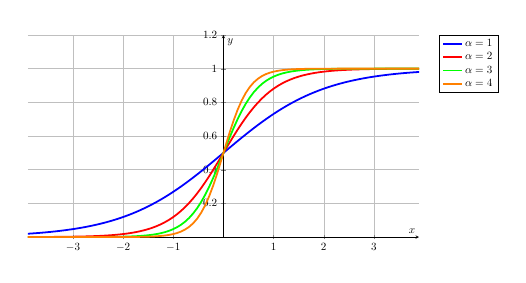
\begin{tikzpicture}[scale=0.4]
            \begin{axis}[
                axis lines=middle,
                xlabel={$x$},
                ylabel={$y$},
                ymin=0, ymax=1.2,
                xmin=-3.9, xmax=3.9,
                domain=-4:4,
                samples=100,
                grid=both,
                width=14cm, % Adjusted for wider aspect ratio
                height=8cm,
                legend style={at={(1.05,1)}, anchor=north west}
            ]
            
            % Plot different sigmoidal functions with bolder lines
            \addplot[ultra thick, blue] {1 / (1 + exp(-1 * x))};
            \addlegendentry{$\alpha=1$}
            
            \addplot[ultra thick, red] {1 / (1 + exp(-2 * x))};
            \addlegendentry{$\alpha=2$}
            
            \addplot[ultra thick, green] {1 / (1 + exp(-3 * x))};
            \addlegendentry{$\alpha=3$}
            
            \addplot[ultra thick, orange] {1 / (1 + exp(-4 * x))};
            \addlegendentry{$\alpha=4$}
        
            \end{axis}
        \end{tikzpicture}

        \footnotesize{\textbf{Рис.}: Логістична функція з різними параметрами $\alpha$.}
        \end{center}
        \end{example}
    \end{frame}

    \begin{frame}{Робота Цибенко (1989)}
        \begin{block}{Апроксимація функцій лінійною комбінацією сігмоїдів}
            Робота Цибенко \cite{cybenko} присвячена на той час відомій апроксимації функції $f:
            \mathbb{R}^m \to \mathbb{R}$ за допомогою наступної суми:
            \begin{equation*}\label{eq:cybenko-g}
                \hat{f}(\boldsymbol{x}) = \sum_{j=1}^n \alpha_j \sigma(\boldsymbol{w}_j^{\top}\boldsymbol{x} + \beta_j), \quad \boldsymbol{w}_j \in \mathbb{R}^m, \quad \alpha_j,\beta_j \in \mathbb{R}.
            \end{equation*}
            \begin{itemize}
                \item По суті, лінійна комбінація виразів $\{\sigma(\boldsymbol{w}_j^{\top}\boldsymbol{x} + \beta_j)\}_{1 \leq j \leq n}$.
                \item $n$ --- кількість нейронів у прихованому шарі.
                \item Маємо рівно $(m+2)n$ параметрів.
            \end{itemize}
            
        \end{block}

        \pause\begin{alertblock}{Питання}
            Який клас функцій може апроксимувати така модель?
        \end{alertblock}
    \end{frame}

    \begin{frame}{Візуалізація Архітектури Цибенко}
        \begin{tikzpicture}[scale=0.8]
            % Define layers and node style
            \tikzset{input-neuron/.style={
                circle, 
                draw=green!80!black, 
                line width=0.5mm,
                fill=green!20!white,
                minimum size=0.5cm
            }}
            \tikzset{hidden-neuron/.style={
                circle, 
                draw=blue!80!black, 
                line width=0.5mm,
                fill=blue!20!white,
                minimum size=0.5cm
            }}
            \tikzset{output-neuron/.style={
                circle, 
                draw=orange!80!black, 
                line width=0.5mm,
                fill=orange!20!white,
                minimum size=0.5cm
            }}
            
            % Input layer
            \foreach \i in {1, 2, 3} {
                \node[input-neuron] (I\i) at (0, -1.25*\i) {$x_{\i}$};
            }
        
            % Hidden layer
            \foreach \j in {1, 2, 3, 4, 5} {
                \node[hidden-neuron] (h\j) at (4, -1.25*\j + 1.25) {$\Sigma$};
                \node[hidden-neuron] (H\j) at (6, -1.25*\j + 1.25) {$z_{\j}$};
                \draw[very thick,-{Stealth[length=3.5mm]}] (h\j) to [edge label=$\sigma$] (H\j);
            }
        
            % Output layer
            \node[output-neuron] (O) at (10, -2.5) {$\hat{f}(\boldsymbol{x})$};
        
            % Draw connections from input to hidden layer
            \foreach \i in {1, 2, 3} {
                \foreach \j in {1, 2, 3, 4, 5} {
                    \draw[very thick,-{Stealth[length=3.5mm]}] (I\i) -- (h\j);
                }
            }
        
            % Draw connections from hidden to output layer
            \foreach \j in {1, 2, 3, 4, 5} {
                \draw[very thick,-{Stealth[length=3.5mm]}] (H\j) -- (O);
            }
        
            % Labels
            \node[above, align=center] at (0, 0.5) {\textcolor{green!80!black}{\textbf{Вхідний шар}}\\$m$ нейронів};
            \node[above, align=center] at (5, 0.5) {\textcolor{blue!80!black}{\textbf{Прихований шар}}\\$n$ нейронів};
            \node[above, align=center] at (10, 0.5) {\textcolor{orange!80!black}{\textbf{Вихідний шар}}\\1 нейрон};
        
        \end{tikzpicture}

        \begin{block}{Зауваження}
            \textbf{Нейрон} --- це просто значення у графі обчислень.
        \end{block}
    \end{frame}

    \begin{frame}{Теорема Цибенко}
        \begin{itemize}
            \item $\mathcal{Q}_m = [0,1]^m$ є $m$-вимірним одиничним гіперкубом.\pause
            \item $\mathcal{C}(\mathcal{Q}_m)$ --- простір неперервних функцій $f: \mathcal{Q}_m \to \mathbb{R}$.\pause
            \item Норма функції $f$ на $\mathcal{C}(\mathcal{Q}_m)$: $\|f\|_{\mathcal{Q}_m} = \sup_{\boldsymbol{x} \in \mathcal{Q}_m} |f(\boldsymbol{x})|$.\pause
        \end{itemize}

        \begin{theorem}[Цибенко]
            Нехай $\sigma$ будь-яка неперервна сігмоїдальна функція. Суми вигляду
            $\hat{f}(\boldsymbol{x}) = \sum_{j=1}^n
            \alpha_j\sigma(\boldsymbol{w}_j^{\top}\boldsymbol{x} + \beta_j)$ є щільними у
            $\mathcal{C}(\mathcal{Q}_m)$ та $L^1(\mathcal{Q}_m)$. Іншими словами, для
            будь-якої функції $f \in \mathcal{C}(\mathcal{Q}_m)$ та $\varepsilon > 0$,
            існує сума $\hat{f}(\boldsymbol{x})$ така, що:
            \begin{enumerate}
                \item $|\hat{f}(\boldsymbol{x})-f(\boldsymbol{x})|<\varepsilon$ для всіх $\boldsymbol{x} \in
                \mathcal{Q}_m$.
                \item $\int_{\mathcal{Q}_m}|\hat{f}(\boldsymbol{x})-f(\boldsymbol{x})|d\boldsymbol{x} <
                \varepsilon$.
            \end{enumerate}
        \end{theorem}

        \pause\begin{alertblock}{Висновок}
            $\sum_{j=1}^n
            \alpha_j\sigma(\boldsymbol{w}_j^{\top}\boldsymbol{x} + \beta_j)$ апроксимує 
            довільну функцію на $\mathcal{C}(\mathcal{Q}_m)$.
        \end{alertblock}
    \end{frame}

    \subsection{Універсальність апроксимації класифікатора}
    \begin{frame}{Чи це все?}
        \begin{alertblock}{Питання}
            Нехай $\mathcal{P}_0,\dots,\mathcal{P}_{C-1}$ ---
            розбиття $\mathcal{Q}_m$ на $C$ підмножин (що називають \textit{класами}).\pause Нехай
            $f: \mathcal{Q}_m \to \{0,\dots,C-1\}$ задана так:
            \begin{equation*}
                f(\boldsymbol{x}) = j \iff \boldsymbol{x} \in \mathcal{P}_j.
            \end{equation*}

            \pause Чи може $\hat{f}(\boldsymbol{x}) := \sum_{j=1}^n
            \alpha_j\sigma(\boldsymbol{w}_j^{\top}\boldsymbol{x} + \beta_j)$ апроксимувати 
            $f$?\pause
        \end{alertblock}

        \begin{theorem}[Цибенко про класифікатор]
            Нехай $\sigma$ будь-яка неперервна сігмоїдальна функція і функція
            $f$ задана як вище. Тоді для будь-якої такої функції існує $\hat{f}$
            та множина $\mathcal{D} \subseteq \mathcal{Q}_m$ така, що міра
            $\mu(\mathcal{D}) \geq 1-\varepsilon$ та $|\hat{f}(\boldsymbol{x}) -
            f(\boldsymbol{x})| < \varepsilon$ для всіх $\boldsymbol{x} \in \mathcal{D}$.
        \end{theorem}
    \end{frame}

    \begin{frame}{Ілюстрація}
        \begin{figure}
        \begin{tikzpicture}
            % Draw the main square [0,1]^2
            \draw[very thick] (0,0) rectangle (4,4);
            
            % Partition the square into regions
            % Region 1
            \fill[red!50,opacity=0.5] (0,0) rectangle (2,2);
            \node[text width=2cm,align=center,red!30!black] at (1,1) {\large $\mathcal{P}_0$:\\ $f(\boldsymbol{x}) \equiv 0$};
            
            % Region 2
            \fill[blue!50,opacity=0.5] (2,0) rectangle (4,2);
            \node[text width=1.75cm,align=center,blue!30!black] at (3,1) {\large $\mathcal{P}_1$:\\ $f(\boldsymbol{x}) \equiv 1$};
            
            % Region 3
            \fill[green!50,opacity=0.5] (0,2) rectangle (4,4);
            \node[text width=3.0cm,align=center,green!30!black] at (2,3) {\large $\mathcal{P}_2: f(\boldsymbol{x}) \equiv 2$};
            
            % Label axes
            \draw[very thick, -{Stealth[length=3.5mm]}] (-0.5,0) -- (4.5,0) node[anchor=north west] {$x$};
            \draw[very thick, -{Stealth[length=3.5mm]}] (0,-0.5) -- (0,4.5) node[anchor=south east] {$y$};
            
            % Add labels for the square boundaries
            \node[below] at (0.25,0.0) {\footnotesize $0$};
            \node[below] at (4,0) {\footnotesize $1$};
            \node[left] at (0,4) {\footnotesize $1$};
        \end{tikzpicture}
        \caption{Розбиття $\mathcal{Q}_2$ на три класи $\mathcal{P}_0,\mathcal{P}_1,\mathcal{P}_2$ (себто, $C=3$).}
        \end{figure}
    \end{frame}

    \begin{frame}{Практична реалізація}
        \begin{alertblock}{Додаток}
            У курсовій роботі ми також написали програму, що для заданого
            бінарного розбиття $\mathcal{P}_0,\mathcal{P}_1$, знаходить
            класифікатор $\hat{f}$.
        \end{alertblock}

        % Show two images side by side using minipage
        \begin{figure}
            \begin{minipage}{0.475\textwidth}
                \centering
                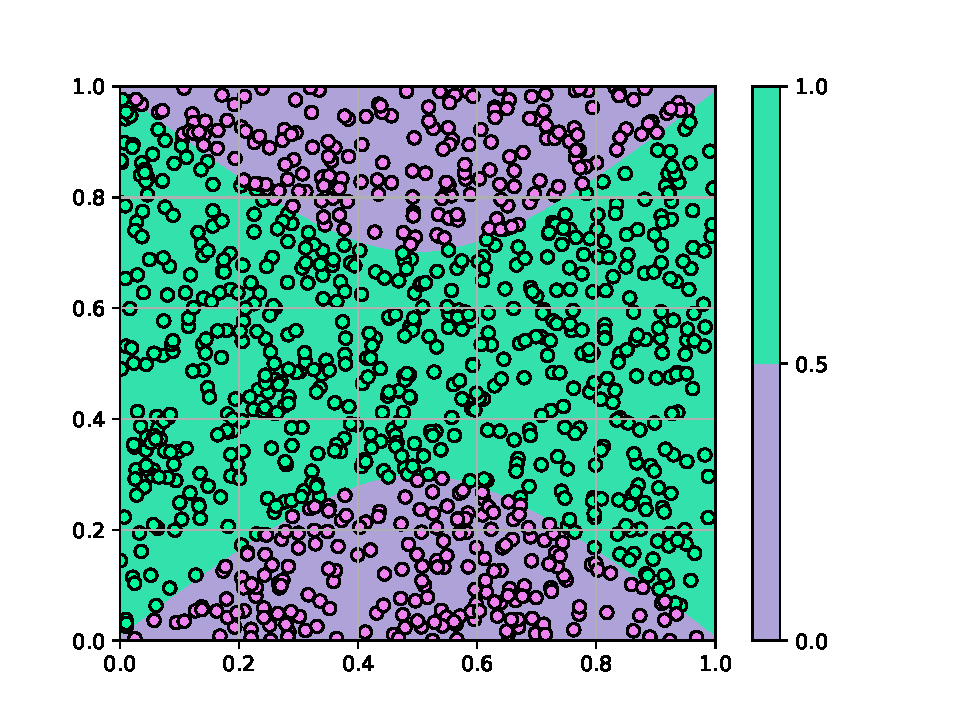
\includegraphics[width=\textwidth]{../code/classification-example.pdf}
                \caption{Правильне розбиття $\mathcal{P}_0,\mathcal{P}_1$.}
            \end{minipage}\hfill
            \begin{minipage}{0.475\textwidth}
                \centering
                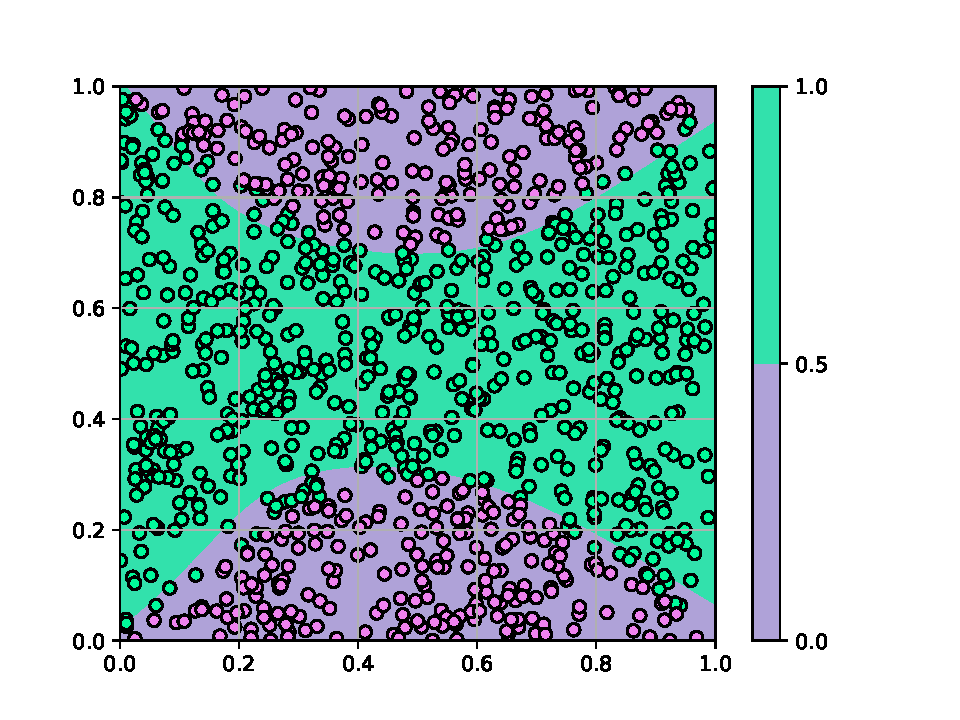
\includegraphics[width=\textwidth]{../code/classification-discr-prediction.pdf}
                \caption{Розбиття, знайдене класифікатором $\hat{f}$.}
            \end{minipage}
        \end{figure}
    \end{frame}

    \begin{frame}{Узагальнення: MLP}
        \begin{enumerate}
            \item Замість сігмоїду $\sigma$, використовуються інші \textbf{нелінійні}
            активаційні функції $\phi: \mathbb{R} \to \mathbb{R}$ (напр., $\phi(x) = \max\{0,x\}$).\pause
            \item Замість двох шарів, може бути довільна кількість шарів.\pause
        \end{enumerate}

        \begin{definition}[Багатошарова модель персептронів (MLP)]\label{def:mlp}
            Таким чином, узагальнена архітектура:
            \begin{equation*}
                \boldsymbol{x}^{\langle j+1 \rangle} = \phi^{\langle j \rangle}(\boldsymbol{z}^{\langle j \rangle}), \quad \boldsymbol{z}^{\langle j \rangle} = \boldsymbol{W}^{\langle j \rangle}\boldsymbol{x}^{\langle j \rangle} + \boldsymbol{\beta}^{\langle j \rangle}, \quad j = 0,\dots,\ell-1,
            \end{equation*}
            Таким чином, параметризація моделі є $\boldsymbol{\theta} =
            \left\{\boldsymbol{W}^{\langle j \rangle},\boldsymbol{\beta}^{\langle j
            \rangle}\right\}_{0 \leq j \leq \ell-1}$.
        \end{definition}

        \begin{alertblock}{Зауваження}
            \pause У курсовій роботі, ми розглянули питання: (a) навіщо потрібно більше двох шарів, (b) які бувають узагальнення архітектури MLP та (c) навіщо інші активаційні функції.
        \end{alertblock}
    \end{frame}

    \section{Мережі Колмогорова-Арнольда}

    \subsection{Історична довідка: 13 проблема Гільберта}
    \begin{frame}{13 проблема Гільберта}
        \begin{alertblock}{Питання}
            Чи існують справжні неперервні функції від багатьох змінних?\pause
        \end{alertblock}

        \begin{alertblock}{Перефразоване питання}
            Чи можна будь-яку неперервну функцію $f: \mathcal{Q}_m \to
            \mathbb{R}$ записати за допомогою суми та композицій
            $\phi_1,\dots,\phi_N \in \mathcal{C}(\mathbb{R})$?\pause
        \end{alertblock}

        \begin{example}
            $f(x,y) = 3x+5y$. Якщо
            $\phi_1(x)=3x$, $\phi_2=5y$, то 
            $f(x,y) = \phi_1(x)+\phi_2(y)$.\pause
        \end{example}

        \begin{example}
            $f(x,y) = xy$. Оскільки $xy=\frac{(x+y)^2}{4} - \frac{(x-y)^2}{4}$, 
            то якщо $\phi(x)=-x,\psi_+(x)=x^2/4,\psi_-(x)=-x^2/4$, то:
            \begin{equation*}
                f(x,y) = \psi_+(x+y) + \psi_-(x+\phi(y)).
            \end{equation*}
        \end{example}
    \end{frame}

    \begin{frame}{Теорема Колмогорова-Арнольда}
        \begin{block}{Основна гіпотеза 13 проблеми Гільберта}
            Існує неперервна функція $f: \mathcal{Q}_3 \to \mathbb{R}$, що не може бути
            виражена як композиція та сума неперервних функцій $\phi_1,\dots,\phi_N \in
            \mathcal{C}(\mathbb{R}^2)$.\pause
        \end{block}

        \begin{definition}[Теорема Колмогорова (1957, \cite{kolmogorov-original})]
            Для будь-якого натурального $m \geq 2$, існують неперервні функції
            $\phi_{p,q} \in \mathcal{C}([0,1])$ такі, що для будь-якої функції $f \in
            \mathcal{C}(\mathcal{Q}_m)$ знайдуться неперервні функції
            $\Phi_1,\dots,\Phi_{2m+1} \in \mathcal{C}(\mathbb{R})$ такі, що
            \begin{equation*}
                f(x_1,\dots,x_m) = \sum_{q=1}^{2m+1}\Phi_q\left(\sum_{p=1}^n \phi_{p,q}(x_p)\right)
            \end{equation*}
        \end{definition}
    \end{frame}

    \subsection{Мережа Колмогорова-Арнольда}
    \begin{frame}{Мережа Колмогорова-Арнольда(KAN)}
        \begin{block}{Зауваження}
            До роботи 2024 року \cite{kan}, ідею такої репрезентації вважали недосяжною через
            ``поганість'' функцій $\phi_{p,q}$ та $\Phi_q$. \pause
        \end{block}

        \begin{definition}[З'єднання KAN Мережі \cite{kan}]
            \textbf{З'єднання KAN Мережі} між шарами розміру $n$ (вхід)
            та $m$ (вихід) --- це матриця $\boldsymbol{\Phi} = \{\phi_{q,p}\}_{1 \leq p \leq n, 1 \leq q \leq m}$, де 
            кожна функція параметризована, а наступне значення активації $\boldsymbol{y} = \boldsymbol{\Phi} \circ \boldsymbol{x}$.\pause
        \end{definition}

        \begin{equation*}
            \begin{bmatrix}
                y_1 \\
                \vdots \\
                y_{m}
            \end{bmatrix} =
            \begin{bmatrix}
                \phi_{1,1} & \cdots & \phi_{1,n} \\
                \vdots & \ddots & \vdots \\
                \phi_{m,1} & \cdots & \phi_{m,n}
            \end{bmatrix}\circ \begin{bmatrix}
                x_1 \\
                \vdots \\
                x_n
            \end{bmatrix} \triangleq \begin{bmatrix}
                \sum_{p=1}^n \phi_{1,p}(x_p) \\
                \vdots \\
                \sum_{p=1}^n \phi_{m,p}(x_p)
            \end{bmatrix}
        \end{equation*}
    \end{frame}

    \begin{frame}{Мережа Колмогорова-Арнольда(KAN), cont.}
        \begin{definition}[Архітектура KAN \cite{kan}]
            \textbf{Мережа Колмогорова-Арнольда} --- це композиція $\ell$ з'єднань:
            \begin{equation*}
                \hat{f}_{\text{KAN}}(\boldsymbol{x}) = \boldsymbol{\Phi}^{\langle \ell-1 \rangle} \circ \cdots \circ \boldsymbol{\Phi}^{\langle 1 \rangle} \circ \boldsymbol{\Phi}^{\langle 0 \rangle} \circ \boldsymbol{x}.
            \end{equation*}
        \end{definition}

        \pause\begin{example}[Формула Колмогорова]
            Нехай $\boldsymbol{\Phi}^{\langle 0 \rangle} = \{\phi_{p,q}\}_{1 \leq p \leq m, 1 \leq q \leq 2m+1}$, $\boldsymbol{\Phi}^{\langle 1 \rangle} = \{\Phi_q\}_{1 \leq q \leq 2m+1}$:
            \begin{align*}
                \small
                \hat{f}_{\text{KAN}}(\boldsymbol{x}) = \begin{bmatrix}
                    \Phi_1, \dots, \Phi_{2m+1}
                \end{bmatrix} \circ \begin{bmatrix}
                    \phi_{1,1} & \cdots & \phi_{1,m} \\
                    \vdots & \ddots & \vdots \\
                    \phi_{2m+1,1} & \cdots & \phi_{2m+1,m}
                \end{bmatrix} \circ \begin{bmatrix}
                    x_1 \\
                    \vdots \\
                    x_m
                \end{bmatrix} \\
                = \small\begin{bmatrix}
                    \Phi_1, \dots, \Phi_{2m+1}
                \end{bmatrix} \circ \begin{bmatrix}
                    \sum_{p=1}^m \phi_{1,p}(x_p) \\
                    \vdots \\
                    \sum_{p=1}^m \phi_{2m+1,p}(x_p)
                \end{bmatrix} = \sum_{q=1}^{2m+1}\Phi_q\left(\sum_{p=1}^m \phi_{q,p}(x_p)\right)
            \end{align*}
        \end{example}
    \end{frame}

    \begin{frame}{Візуалізація}
        \begin{figure}
            % Include figure
            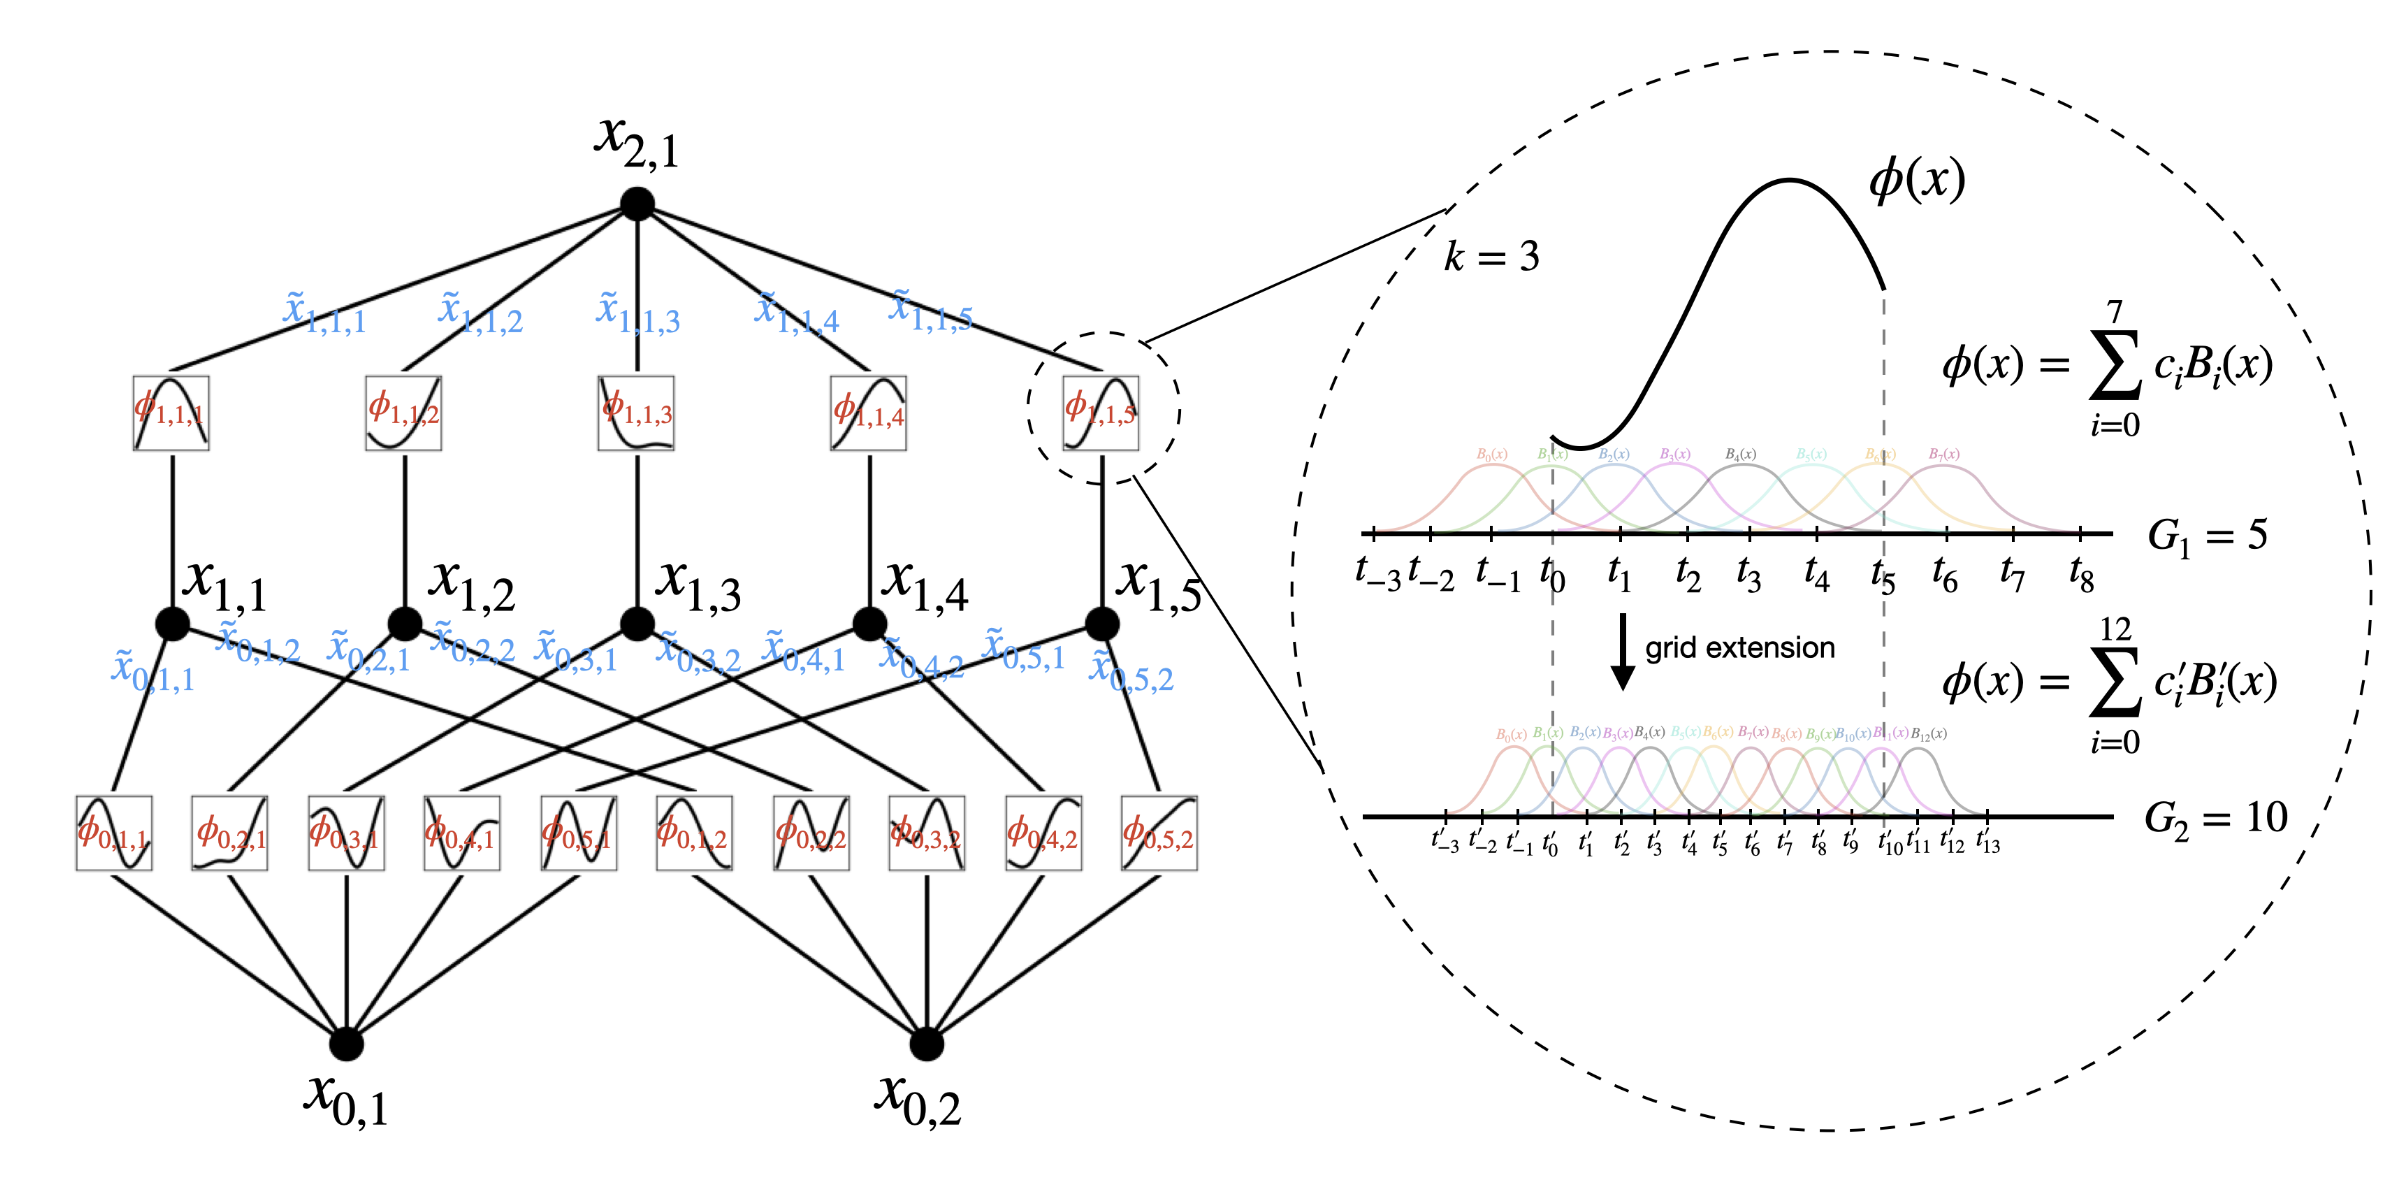
\includegraphics[width=\textwidth]{images/kan.png}
            \caption{Архітектура мережі Колмогорова-Арнольда з оригінальної роботи \cite{kan}.}
        \end{figure}
    \end{frame}

    % \begin{frame}{Порівняння з MLP}
    %     \begin{enumerate}
    %         \item \textbf{Кількість інструментів.} MLP мережі більш розвинуті, 
    %         отже є більш популярними та зручними для використання.\pause
    %         \item \textbf{Швидкість тренування.} Згідно з роботою \cite{kan}, KAN мережі
    %         поки приблизно в $10\times$ повільніші за MLP під час тренування.\pause
    %         \item \textbf{Швидкість передбачення.} Якщо $\ell$ --- кількість шарів,
    %         $d$ --- степінь активаційної функції, то з'єднання $n \times n$ для
    %         MLP вимагає $\mathcal{O}(\ell n^3 d)$ операцій, у той час як для KAN
    %         вимагає $\mathcal{O}(\ell n^2 d)$ операцій.\pause
    %         \item \textbf{Кількість параметрів.} Для MLP маємо
    %         $\mathcal{O}(n^2\ell)$ параметрів, у той час як KAN вимагає
    %         $\mathcal{O}(n^2\ell d)$. 
    %     \end{enumerate}
    % \end{frame}

    \begin{frame}[allowframebreaks]{Література}
        % This prints the bibliography on the slide
        \printbibliography
    \end{frame}

    \begin{frame}[plain, standout]
      \centering
      \LARGE
      \textbf{Дякую за Вашу Увагу!} \\
      
      \vspace{0.2cm} \Huge \ding{170} \large \\
    \end{frame}

    \begin{frame}{Додаткові відомості}
        \begin{definition}[Міра]
            \textbf{Мірою} $\mu$ називають невід'ємну $\sigma$-адитивну функцію 
            множин, задана на півкільці $\mathcal{H}$:
            \begin{itemize}
                \item \textbf{Невід'ємна:} $\forall X \in \mathcal{H}: \mu(X) \geq 0$.
                \item \textbf{$\sigma$-адитивність:} $\forall \{X_n\}_{n \in \mathbb{N}} \subset \mathcal{H}$ таких, що $\{X_n\}_{n \in \mathbb{N}}$ є неперетинними та $\bigcup_{n \in \mathbb{N}}X_n \in \mathcal{H}$, справедливо:
                \begin{equation*}
                    \mu\left(\bigcup_{n \in \mathbb{N}}X_n\right) = \sum_{n \in \mathbb{N}}\mu(X_n).
                \end{equation*}
            \end{itemize}
        \end{definition}
    \end{frame}

    \begin{frame}{Додаткові відомості}
        \begin{definition}[$L^p$ простір]
            \textbf{$L^p$ простором} ($p \geq 1$) над простором з мірою $(\Omega,\mathcal{F},\mu)$ називають множину 
            функцій $\mathcal{L}^p(\Omega,\mu)$, на яких інтеграл Лебега в $p$-ому степені модуля є скінченним:
            \begin{equation*}
                \mathcal{L}^p(\Omega,\mu) = \left\{f: \text{$\mathcal{F}$-вимірна}: \|f\|_p = \left(\int_{\Omega}|f|^pd\mu\right)^{1/p} < \infty\right\}.
            \end{equation*}

            Для $p=\infty$, $\|f\|_{\infty} = \inf\{\gamma \in \mathbb{R}_{\geq 0}: |f(x)| \leq \gamma \; \text{майже для всіх $x \in \Omega$}\}$.
        \end{definition}
    \end{frame}
\end{document}